\documentclass[atiam, article]{rapport} % draft, phelma_black, phelma_normal, kit_de, kit_en, phelma_old
\usepackage{booktabs}

\doctitle{TP Percussions}
\title{TP Percussions\\Accord ou pas d'accord ?}
\titleheader{TP Percussions}
\titleone{}
\titletwo{Acoustique}
\titlethree{}
\author{Paul Estève, Étienne André} % Authors for the header
\autpage{ % Authors for the title page
  \begin{tabular}{l}
    Paul Estève \\
    Étienne André
  \end{tabular}
}
\supervisor[Encadrants : ]{Jean-Loïc Le Carrou\\Christophe Vergez
}
% \supervisorMail{}
\serie{ATIAM 2023/2024}
\date{\today}

\begin{document}

\maketitle

\section{Préparation du TP}

\subsection{Protocole de mesures}
Nous chercherons à mesurer individuellement le comportement de différents instruements après excitation. Nous utiliserons un microphone pour mesurer le champ de pression rayonné. On analysera également en temps réel le son capté avec un spectrogramme et un vu-mètre pour surveiller tout bruit parasite ou saturation.

Afin de disposer d'un éventail de mesures pour chacun des instruments, nous prendrons des mesures de manière uniforme sur sa tessiture, en prenant soin d'inclure les extrêmes. Nous choisirons des points d'excitations représentatifs du jeu d'un percussionniste, et les mailloches typiquement utilisées sur ces instruments.

\begin{itemize}
  \item Vibraphone: point d'excitation au centre de la lame, mailloches de dureté moyenne.
  \item Glockenspiel: point d'excitation au centre de la lame, mailloches dures.
  \item Timbale: point d'excitations du bord jusqu'au centre de la membrane, mailloches souples.
\end{itemize}


Pour le glockenspiel et le vibraphone, le micro sera déplacé pour chaque mesure, dirigé vers le milieu de la lame, à distance fixe.

Pour la timbale, nous envisageons de tester le placement du micro en situation réelle.

\subsection{Reproductibilité de l'excitation}
Afin d'obtenir la même excitation pour toutes les mesures, nous enviseageons de laisser la mailloche pivoter entre nos doigts sous l'effet de la gravité, depuis le même angle et la même position.

\section{Modifications du protocole de mesure}

\subsection{Placement du micro pour la timbale}

Afin de déterminer le meilleur placement de micro, nous avons effectué une mesure préliminaire avec une excitation aux 3/4 du rayon de la membrane. Le micro a été placé successivement
\begin{itemize}
  \item au-dessus centre de la membrane
  \item au-dessus de la moitié du rayon de la membrane, opposé au point de frappe
\end{itemize}
En frappant près du bord de la membrane, la timbale est assimilable à un dipôle rayonnant. On observe donc des annulations dans le spectre lorsque le micro est placé au centre. On placera donc dans la suite le micro dans la seconde position.

\subsection{Reproductibilité de l'excitation}

Après quelques essais, il s'est avéré que notre méthode d'excitation ne convenait pas:
\begin{itemize}
  \item les frottements entre les doigts et la baguette de la mailloche rendent sa vitesse de chute dépendante du serrage des doigts
  \item il est difficile de s'assurer un coup unique et n'amortissant pas l'instrument, la mailloche ne rebondissant qu'assez peu sur l'instrument
\end{itemize}

Face à ces limitations, nous avons choisi de frapper "à la main". Afin que les excitations soient les plus proches d'un dirac, nous veillons à respecter les mouvements en usage chez les percussionistes, notamment exagérer les mouvements pré- et post-frappe, et utiliser les doigts et le poignet plutôt que les avant-bras.

Pour s'assurer d'une forme de similarité entre toutes les frappes, on surveillera également le niveau de pic maximal grâce à un vu-mètre. Cependant, dans la suite, les amplitudes ne seront pas absolument comparées d'un endroit de la tessiture à l'autre, ainsi une petite disparité d'amplitude est acceptable.

\section{Instruments à lames: Vibraphone et Glockenspiel}
\subsection{Étude théorique}

En modélisant une lame par une poutre libre-libre de matériau isotrope et de section uniforme dans les hypothèses d'Euler-Bernouilli, celle-ci est régie par l'équiation suivante:

$$E I \frac{\partial^4 y}{\partial x^4} + \rho S \frac{\partial^2 y}{\partial t^2} $$
où:
\begin{itemize}
  \item $E$ est le module d'Young du matériau
  \item $I$ est le moment d'inertie
  \item $\rho$ est la densité surfacique de la section
  \item $S$ est la section de la poutre
\end{itemize}

\subsection{Inharmonicité des modes}

On montre que les pulsations modales sont $\omega_n = (\beta_n L)^2 \sqrt{\frac{EI}{\rho L}}$ , où:
\begin{itemize}
  \item $L$ est la longueur de la lame.
  \item $\beta_n$ est solution de $\cos{(\beta_n L)} \cosh{(\beta_n L)} = 1$
\end{itemize}

On a donc la relation $\omega_n = \frac{(\beta_n L)^2}{(\beta_1 L)^2} \omega_1$, dont on calcule numériquement les premières valeurs:
\begin{center}
  \begin{tabular}{ c|c|c|c|c|c|c|c|c } 
    $n$ & 0 & 1 & 2 & 3 & 4 & 5 & 6 & 7 \\
    \hline
    $\beta_n L$ & 0.00 & 4.73 & 7.85 & 11.00 & 14.14 & 17.28 & 20.42 & 23.56 \\
    \hline
    $\frac{\omega_n}{\omega_1}$ & - & 1.00 & 2.76 & 5.40 & 8.93 & 13.34 & 18.64 & 24.81 \\
  \end{tabular}
  \label{table:ratios}
\end{center}

\subsection{Amortissement}

Les lames étant métalliques, les pertes thermo-élastiques sont importantes. Le modèle sans perte ci-dessus peut être adapté en considérant le modèle d'Young complexe et dépendant de $\omega$. On s'attendra donc à observer une décroissance exponentielle de l'amplitude de chaque mode.

\subsection{Traitement des mesures}

Un programme python donné en annexe traite chaque mesure et effectue les opérations suivantes:
\begin{itemize}
  \item Détection du transitoire
  \item Mesure du niveau de bruit de fond avant l'attaque
  \item Réduction du signal à sa partie en oscillation libre (choisi comme étant 0.5s après le transitoire jusqu'au moment où le son atteint le niveau de bruit de fond)
  \item Calcul du spectre
  \item Alignement des fréquences relevées visuellement avec les pics
  \item Calcul des amplitudes et facteurs d'harmonicité des partiels
  \item Tracé des figures et tables incluses dans ce rapport
\end{itemize}

Les partiels retenus ont été choisis par nos soins visuellement à l'aide du logiciel Sonic Visualiser, aucune méthode d'analyse automatique n'ayant donné de résultats satisfaisants.

\subsection{Commentaires sur le glockenspiel}
Les spectres des enregistrements et tables d'inharmonicité sont relevés en annexe \ref{annexe:glock}.

On effectue 3 mesures des notes F5, F6 et F7; F5 et F7 étant les extrêmes de la tessiture de l'instrument.

On observe les points suivants:
\begin{itemize}
  \item En comparant les ratios avec ceux données dans la table \ref{table:ratios}, on retrouve les partiels dont l'inharmonicité est prévue par le modèle théorique.
  \item Selon les notes jouées, d'autres partiels sont également présents. Cela montre les limites du modèle qui prend en compte ni la torsion, ni la traction-compression, et ce dans une seule dimension.
\end{itemize}

\subsection{Commentaires sur le vibraphone}
Les spectres des enregistrements et tables d'inharmonicité sont relevés en annexe \ref{annexe:vibra}.

On procède de même sur le vibraphone, où on mesure les lames F3, A4 et E6, F3 et E6 étant les extrêmes de la tessiture de l'instrument. En réalité, la note la plus haute est F6, mais sur l'instrument mis à disposition cette note est amortie par une suspension trop serrée.

Nous mesurons également deux excitations différentes pour A4: au centre et au bord. Lors d'un jeu à 4 baguettes, certains accords sont très difficiles à jouer en frappant au centre des lames sans se contortionner. Le percussionniste préfère alors une position de jeu plus confortable et va frapper certaines lames sur leur bord, afin de garder ses poignets dans la continuité de ses avant-bras.

Cet instrument se distingue du glockenspiel par ses lames usinées qui ne sont donc plus strictement parallélépipédiques, ce afin notamment d'améliorer leur harmonicité.

On observe les points suivants:
\begin{itemize}
  \item Frapper au bord ou au centre ne change pas significativement le spectre rayonné.
  \item Une majorité de partiels sont harmoniques, ce qui confère une sensation de hauteur au vibraphone plus marquée que pour le glockenspiel. Cependant, sur F3, on observe une détérioration de l'harmonicité ainsi que plusieurs partiels manquants.
  \item On ne retrouve pas les partiels "parasites" présents sur le glockenspiel, ce qui peut s'expliquer également par l'usinage des lames.
\end{itemize}

\section{Timbale}


\appendix
\section{Mesures glockenspiel}
\label{annexe:glock}

\begin{figure}[h!]
  \begin{center}
      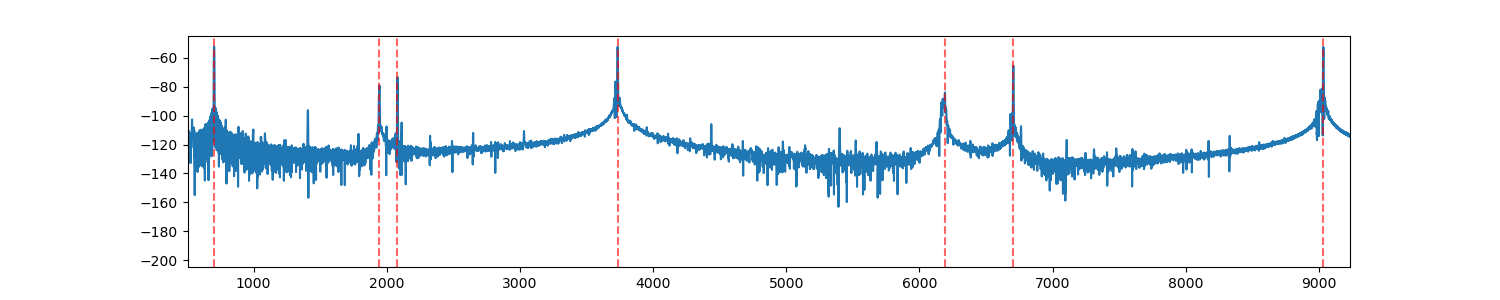
\includegraphics[width=\textwidth]{percu/glock-f5.wav.spectre.png}
  \end{center}
  \caption{Spectre de glock-f5}
\end{figure}
\begin{figure}[h!]
  \begin{center}
      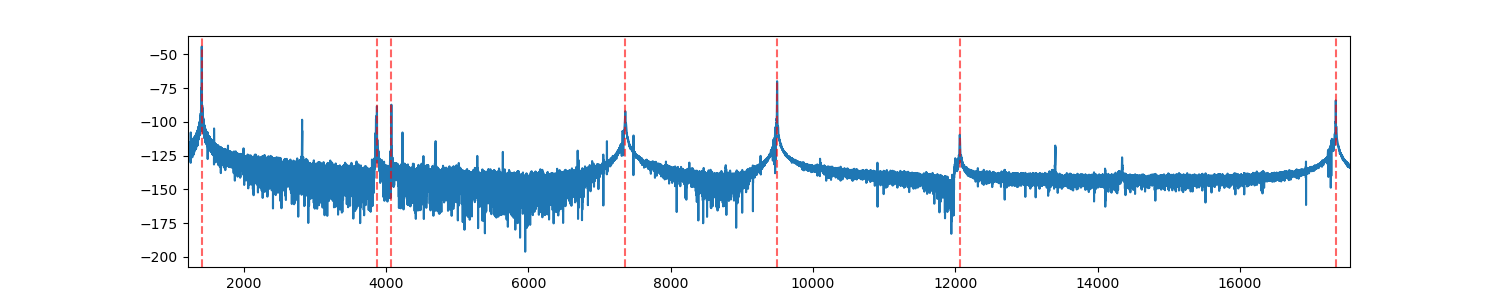
\includegraphics[width=\textwidth]{percu/glock-f6.wav.spectre.png}
  \end{center}
  \caption{Spectre de glock-f6}
\end{figure}
\begin{figure}[h!]
  \begin{center}
      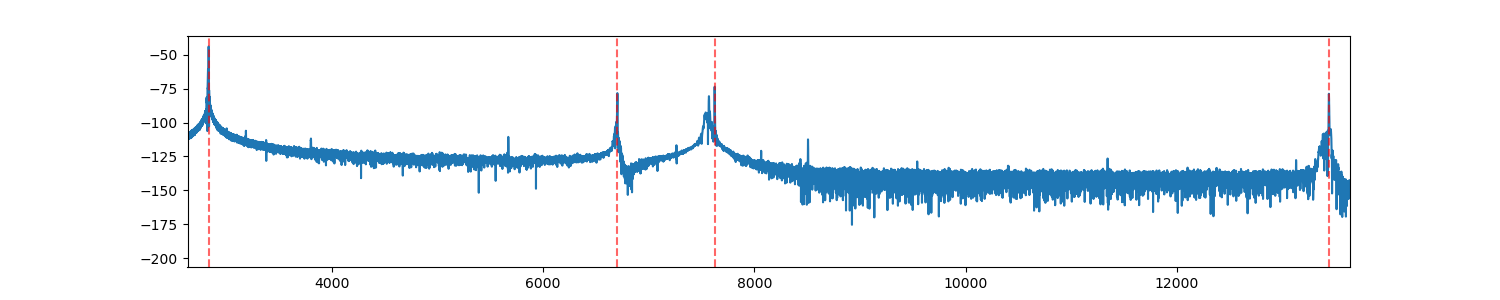
\includegraphics[width=\textwidth]{percu/glock-f7.wav.spectre.png}
  \end{center}
  \caption{Spectre de glock-f7}
\end{figure}

\begin{table}
\centering
\caption{Partiels de glock-f5}
\label{table:partiels-glock-f5.wav}
\begin{tabular}{lrr}
\toprule
{} &  Fréquence (Hz) &  Ratio d'harmonicité \\
\midrule
0 &          703.86 &                 1.00 \\
1 &         1945.13 &                 2.76 \\
2 &         2080.63 &                 2.96 \\
3 &         3737.37 &                 5.31 \\
4 &         6191.16 &                 8.80 \\
5 &         6704.96 &                 9.53 \\
6 &         9033.14 &                12.83 \\
\bottomrule
\end{tabular}
\end{table}

\begin{table}
\centering
\caption{Partiels de glock-f6}
\label{table:partiels-glock-f6.wav}
\begin{tabular}{lrr}
\toprule
{} &  Fréquence (Hz) &  Ratio d'harmonicité \\
\midrule
0 &         1410.64 &                 1.00 \\
1 &         3872.59 &                 2.75 \\
2 &         4075.74 &                 2.89 \\
3 &         7363.04 &                 5.22 \\
4 &         9496.31 &                 6.73 \\
5 &        12063.45 &                 8.55 \\
6 &        17347.69 &                12.30 \\
\bottomrule
\end{tabular}
\end{table}

\begin{table}
\centering
\caption{Partiels de glock-f7}
\label{table:partiels-glock-f7.wav}
\begin{tabular}{lrr}
\toprule
{} &  Fréquence (Hz) &  Ratio d'harmonicité \\
\midrule
0 &         2835.94 &                 1.00 \\
1 &         6704.22 &                 2.36 \\
2 &         7624.69 &                 2.69 \\
3 &        13437.56 &                 4.74 \\
\bottomrule
\end{tabular}
\end{table}


\newpage
\section{Mesures vibraphone}
\label{annexe:vibra}
\begin{figure}[h!]
  \begin{center}
      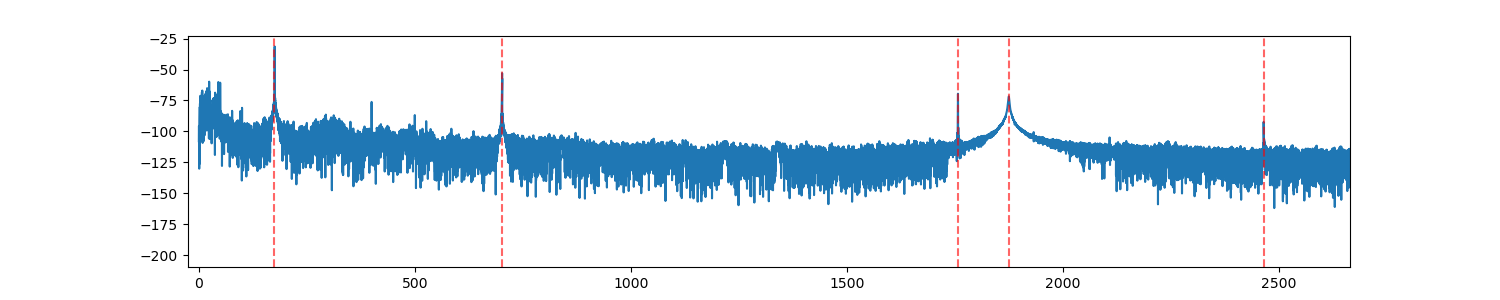
\includegraphics[width=\textwidth]{percu/vibra-f3.wav.spectre.png}
  \end{center}
  \caption{Spectre de vibra-f3}
\end{figure}
\begin{figure}[h!]
  \begin{center}
      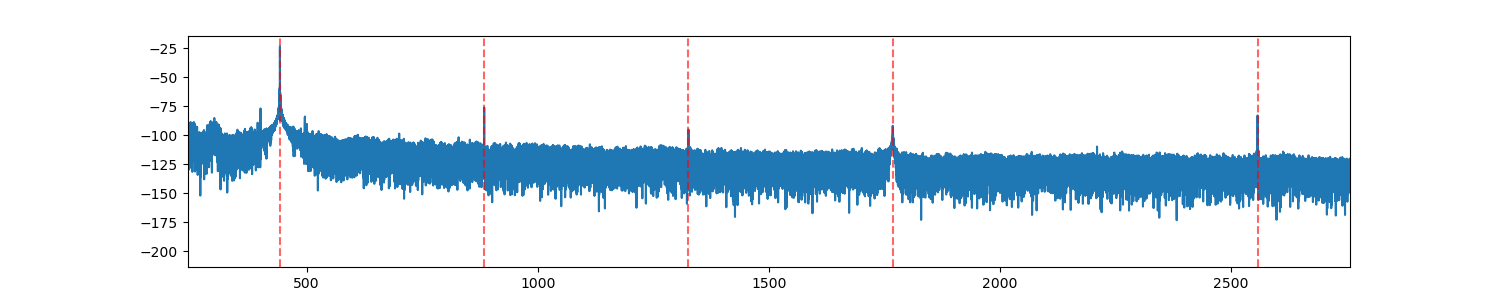
\includegraphics[width=\textwidth]{percu/vibra-a4-centre.wav.spectre.png}
  \end{center}
  \caption{Spectre de vibra-a4-centre}
\end{figure}
\begin{figure}[h!]
  \begin{center}
      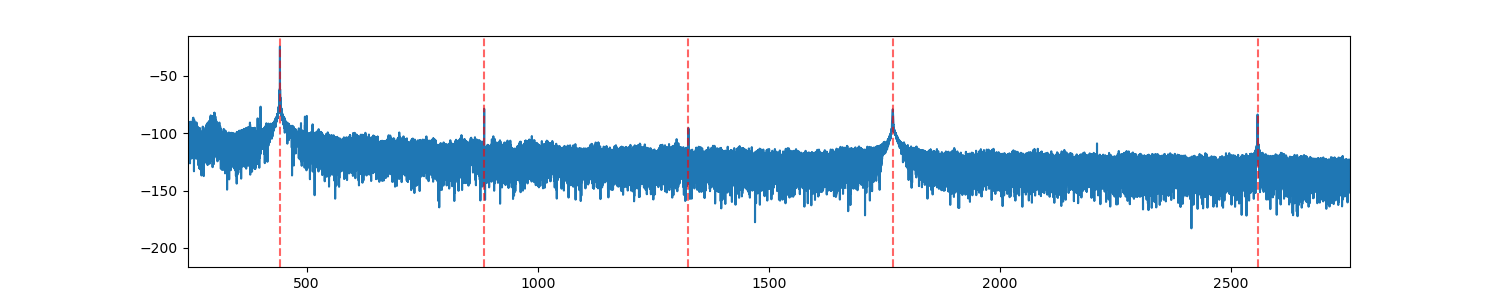
\includegraphics[width=\textwidth]{percu/vibra-a4-bord.wav.spectre.png}
  \end{center}
  \caption{Spectre de vibra-a4-bord}
\end{figure}
\begin{figure}[h!]
  \begin{center}
      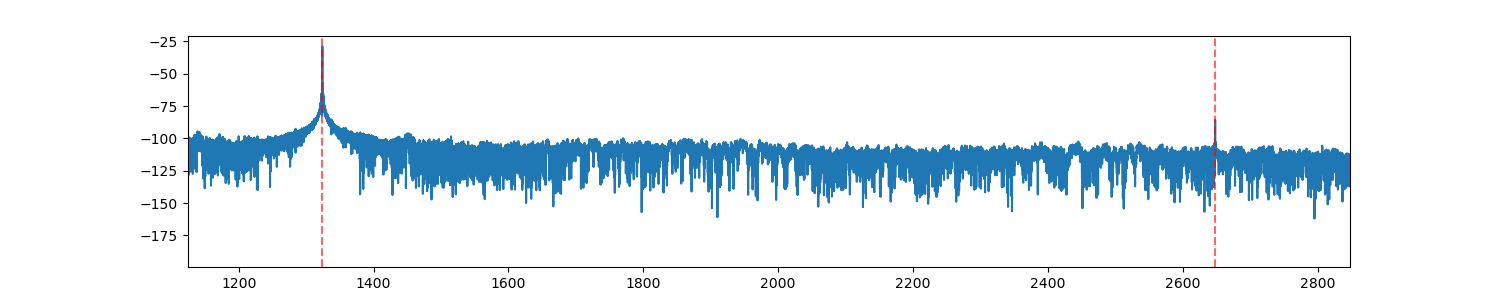
\includegraphics[width=\textwidth]{percu/vibra-e6.wav.spectre.png}
  \end{center}
  \caption{Spectre de vibra-e6}
\end{figure}
\begin{table}
\centering
\caption{Partiels de vibra-f3}
\label{table:partiels-vibra-f3.wav}
\begin{tabular}{lrr}
\toprule
{} &  Fréquence (Hz) &  Ratio d'harmonicité \\
\midrule
0 &          173.69 &                 1.00 \\
1 &          702.91 &                 4.05 \\
2 &         1757.61 &                10.12 \\
3 &         1875.26 &                10.80 \\
4 &         2465.31 &                14.19 \\
\bottomrule
\end{tabular}
\end{table}

\begin{table}
\centering
\caption{Partiels de vibra-a4-bord}
\label{table:partiels-vibra-a4-bord.wav}
\begin{tabular}{lrr}
\toprule
{} &  Fréquence (Hz) &  Ratio d'harmonicité \\
\midrule
0 &          442.01 &                 1.00 \\
1 &          884.02 &                 2.00 \\
2 &         1326.02 &                 3.00 \\
3 &         1768.08 &                 4.00 \\
4 &         2557.45 &                 5.79 \\
\bottomrule
\end{tabular}
\end{table}

\begin{table}
\centering
\caption{Partiels de vibra-a4-centre}
\label{table:partiels-vibra-a4-centre.wav}
\begin{tabular}{lrr}
\toprule
{} &  Fréquence (Hz) &  Ratio d'harmonicité \\
\midrule
0 &          442.01 &                 1.00 \\
1 &          884.03 &                 2.00 \\
2 &         1326.03 &                 3.00 \\
3 &         1767.95 &                 4.00 \\
4 &         2557.45 &                 5.79 \\
\bottomrule
\end{tabular}
\end{table}

\begin{table}
\centering
\caption{Partiels de vibra-e6}
\label{table:partiels-vibra-e6.wav}
\begin{tabular}{lrr}
\toprule
{} &  Fréquence (Hz) &  Ratio d'harmonicité \\
\midrule
0 &         1324.00 &                 1.00 \\
1 &         2648.00 &                 2.00 \\
\bottomrule
\end{tabular}
\end{table}


\end{document}
